% for sublime text 3
%!TEX root = diss.tex

\chapter{Lexical Cohesion Graph}
\label{ch:lex-graph}

An essential type of relations across sentences in a text is the semantic relationships among words of sentences. 
This type of connectivity in text processing is known as lexical cohesion. 
In this chapter, we devise a method for identifying and representing lexical cohesion in texts. 
We first motivate the usage of lexical relations in a text for coherence modeling (Section \ref{sec:lex-graph-motivation}). 
We then explain a graph-based approach for modeling lexical relations among sentences in a text (Section \ref{sec:lex-graph-representation}). 
We employ a sampling method for extracting subgraphs from graph representations of texts (Section \ref{sec:lex-graph-pattern-mining}). 
We explain the sparsity problem related to the frequencies of subgraphs and then adapt a solution from statistical language modeling methods for this problem for graphs (Section \ref{sec:lex-graph-smoothing}). 
We assess the lexical cohesion graph representations of texts and the impacts of the smoothing method on two datasets for the readability assessment task (Section \ref{sec:lex-graph-results}). 
Finally, we provide a summary of the research in this chapter (Section \ref{sec:lex-graph-summary}).

\section{Lexical Cohesion}
\label{sec:lex-graph-motivation}

Coherent texts are beyond arbitrary choices of words and sentences.  
In such texts, sentences are related to each other to smooth the flow of information in texts. 
As we discussed in Chapter~\ref{ch:coherence}, this is achieved through cohesive semantic relations that are expressed through the grammar and the vocabulary of a language \cite{halliday76}. 
The former is referred to as grammatical local coherence and the latter as lexical cohesion. 
Here we focus on lexical cohesion, which comprises one of the semantic connections among words in a text \cite{hoey91}. 

The basis of lexical cohesion is, in fact, extended to any pair of lexical items that stand next to each other in some lexico-semantic relations. 
Some examples of such relations are as follows\footnote{We refer readers for more information to Chapter \ref{ch:coherence} and Chapter \ref{ch:rel-work}.}:  

\begin{itemize}

\item Repetition, which happens when a word in a sentence is repeated in another sentence; 


\item Synonymy, which happens when a word in a sentence means exactly or nearly the same as a word in another sentence. 
For example, verbs ``buy'' and ``purchase'' have a synonymy relationship with each other;  

\item Hyperonymy, which shows the relationship between a generic word (hypernym) in a sentence and a specific instance of it (hyponym) in another sentence. 
For example, there exist a hyperonymy relationship between words ``red'', ``blue'' and ``color'';

\item Meronymy, which happens when a word in a sentence is a constituent part of or a member of the concept that is mentioned by a word in another sentence. 
For example, ``finger'' and ``hand'' are in the meronymy relationship because a finger is part of a hand;

\item Antonymy, which occurs when two words are semantically opposite to each other, e.g.,\ words ``willing'' and  ``reluctant'' are an antonym of each other. 

\item Collocation, which happens when two words frequently occur in the same context together. As an example, words ``doctor'' and ``patient'' are semantically related just because they are frequently used together.

\end{itemize}

An essential property of lexical relations is that lexical items should not necessarily have the same reference in order to relate two sentences \cite{halliday76}.
Consider the sample text\footnote{Taken from the \emph{Cohesion in English} book written by \newcite{halliday76}.} that is presented in Example \ref{ex:lex-graph-boy-girl-text}.

\begin{examples}
  \label{ex:lex-graph-boy-girl-text}
  Why does the little \textbf{boy} wriggle all the time? \\
  \textbf{Girls} don't.
\end{examples}

The lexical items ``boy'' and ``girls'' do not refer to the same entity but they make these two sentences related because they are semantically related.  

In order to recognize lexical semantic relations between words, a lexical knowledge resource is needed.   
One option is to use a lexical resource such as WordNet \cite{fellbaum98} or Freebase \cite{bollacker08}.  
This option is expensive in terms of determining the best resource.  
WordNet lacks a broad coverage in particular with proper names, and Freebase is restricted to nominal concepts and entities. 
Besides, this type of resources is rarely available for other languages than English.
If they are available, their coverage is not as broad as their versions for English. 
Almost none of the available non-English WordNet resources comes close to WordNet's size and coverage on English. 
The other alternative for identifying lexical relations is to employ a set of pre-trained word embeddings. 
Word embeddings which are trained on large corpora of texts can capture word relationships in a language. 
Embedding representations of words give the model the capability to efficiently encode semantic relations among lexical items in a vector space. 
Words that are semantically related in the text space, their embeddings are similar to each other in the vector space. 
Therefore, the semantic relations between words can simply be measured by the cosine function over the angle between the corresponding word vectors. 
It is worth to mention that such word vectors can be easily trained for any language if a large corpus of texts on the language is available (see more about word embeddings in Chapter~\ref{ch:rel-work}).  

In the research presented in this thesis, we use word embeddings to check whether there exists a relationship between two words or not.  
There is no straight way to determine the type of a relation between two words by means of the cosine function. 
However, this is something that we do not need for the purpose of research in this thesis. 
\newcite{halliday76} argue that for the texture purposes, it is only necessary to recognize lexical items that are related. 

\section{LexGraph}
\label{sec:lex-graph-representation}

Since graph representations of entity-based relations across sentences in a text have been shown useful for modeling coherence (see Chapter \ref{ch:coh-patterns}), we focus on providing a graph representation of lexical semantic relations across sentences in a text. 
This graph is built on the existence of lexical relations among words in sentences. 
In the research in this dissertation, we refer to this graph representation of a text as lexical cohesion graph or \emph{LexGraph}. 

More formally, LexGraph $G=<V,E>$ comprises two sets: $V$ is a set of nodes representing sentences in a text, and $E$ is a set of directed edges. 
The direction of an edge between two nodes indicates the order of the sentences that are associated with the nodes. 
The edge itself represents the existence of two word vectors with high cosine similarity, which is a proxy of a lexical semantic relation between words and therefore their corresponding sentences. 

Inspired by the lexical cohesion theory \cite{halliday76}, two sentences are semantically connected if there exists at least one semantic relation between a pair of words in the sentences. 
Semantic relations between words are modeled by their corresponding \mbox{pre-trained} word embeddings.  
Given word vector $\vec{v}_i$ for word $w_i$ and word vector $\vec{v}_j$ for word $w_j$, the value of the cosine metric between these two word vectors, $\mathtt{cos}(\vec{v}_i,\vec{v}_j)$, measures the strength of the relation between word $w_i$ and word $w_j$. 
The range of the cosine metric is in the interval $\left[ -1, +1 \right]$.  
One interpretation of the cosine metric is the normalized correlation coefficient of its inputs.
This metric quantifies the relatedness between the words associated with two input word vectors \cite{manning99}. 
The absolute value of the cosine metric, $|\mathtt{cos}(\vec{v}_i,\vec{v}_j)|$, encodes how strongly two words are related.  

Figure \ref{fig:lex-graph-lexgraph} illustrates our approach to model the connection between two sentences as an edge in a LexGraph. 

\begin{figure}[!ht]
  \begin{center}
      \begin{tabular}{c}
          \begin{tikzpicture}
            \tikzstyle{word}=[circle,thick,draw=black!75,fill=black!10,minimum size=2mm]
            \tikzstyle{sent}=[ellipse, draw, minimum height=1.5cm]
            \tikzstyle{edge}=[draw, dashed,-]
            \begin{scope}  
              \node [word] (w1) at (0,0) {\tiny{$w_1$}};
              \node [word] (w2) at (2,0) {\tiny{$w_2$}};
              \node [word] (w3) at (4,0) {\tiny{$w_3$}}; 
              \node[sent, minimum width=6cm]  (A) at (2,0) {};
              \node  (A) at (2,-1.25) {$(A)$};

              \node [word] (w4) at (8,0) {\tiny{$w_4$}}; 
              \node [word] (w5) at (10,0) {\tiny{$w_5$}}; 
              \node[sent, minimum width=3cm ] (B) at (9,0) {};
              \node  (B) at (9.8,-1.25) {$(B)$};

            \end{scope}    
        \end{tikzpicture}
        \\
          (a)
        \\
        \begin{tikzpicture}
            \tikzstyle{word}=[circle,thick,draw=black!75,fill=black!10,minimum size=2mm]
            \tikzstyle{sent}=[ellipse, draw, minimum height=1.5cm]
            \tikzstyle{edge}=[draw, dashed,-]
            \begin{scope}  
              \node [word] (w1) at (0,0) {\tiny{$\vec{v}_1$}};
              \node [word] (w2) at (2,0) {\tiny{$\vec{v}_2$}};
              \node [word] (w3) at (4,0) {\tiny{$\vec{v}_3$}}; 
              \node[sent, minimum width=6cm]  (A) at (2,0) {};
              \node  (A) at (2,-1.25) {$(A)$};

              \node [word] (w4) at (8,0) {\tiny{$\vec{v}_4$}}; 
              \node [word] (w5) at (10,0) {\tiny{$\vec{v}_5$}}; 
              \node[sent, minimum width=3cm ] (B) at (9,0) {};
              \node  (B) at (9.8,-1.25) {$(B)$};

              \path[edge , bend right=60] (w4) edge [above] node[font=\tiny] {} (w1);
              \path[edge, bend right=60, solid] (w4) edge [above] node[font=\tiny] {} (w2);
              \path[edge, bend right=60] (w4) edge [above] node[font=\tiny] {} (w3);
            
              \path[edge ,bend left=60] (w5) edge [above] node[font=\tiny] {} (w1);
              \path[edge,bend left=60] (w5) edge [above] node[font=\tiny] {} (w2);
              \path[edge,bend left=60, solid] (w5) edge [above] node[font=\tiny] {} (w3);
            \end{scope}        
      \end{tikzpicture}
      \\
      (b)
    \end{tabular}
  \end{center}
  \caption{
  (a) Sentence $A$ with three words $\lbrace w_1,w_2,w_3 \rbrace$ precedes sentence $B$ with two words $\lbrace w_4,w_5 \rbrace$.  
  (b) Words of sentences are replaced by their associated \mbox{pre-trained} word embeddings. 
  Different type of connections represents various edge weights, i.e.,\ the cosine metric between vector pairs. 
  Solid edges have higher weights than dashed edges.  
  The cosine metric of $\vec{v}_4$ and $\vec{v}_2$ is the highest among all edges that are connected to $\vec{v}_4$. 
  The same interpretation holds for the connection between $\vec{v}_5$ and $\vec{v}_3$.
  } 
  \label{fig:lex-graph-lexgraph}
\end{figure}

The connection between two sentences is defined based on the lexical relations among words in the sentences. 
Assume sentence $A$ with three words $\lbrace w_1,w_2,w_3 \rbrace$ precedes sentence $B$ with two 
words $\lbrace w_4, w_5 \rbrace$ in a text.  
Words in the sentences are mapped to their associated pre-trained word embeddings. 
Vectors $\lbrace \vec{v}_1,\vec{v}_2,\vec{v}_3 \rbrace$ are word embeddings associated with words in sentence $A$ and vectors $\lbrace \vec{v}_4, \vec{v}_5 \rbrace$ represent words in sentence $B$. 
For each word in $B$, we compute its relatedness with any word in sentence $A$ by computing the absolute value of the cosine function between the embeddings of words.  
We consider $|\mathtt{cos}(\vec{v}_j,\vec{v}_i)|$ as the weight of the edge that connects vector $\vec{v}_j$ in $B$ to vector $\vec{v}_i$ in $A$.  
Finally, the edge with the maximum weight is selected to capture the lexical relation between word $w_j$ in sentence $B$ with the most semantically related word in sentence $A$. 
More concretely, word $w_j$ in sentence $B$ is connected with word $w_i^\ast$ in sentence $A$ such that 

\begin{equation}
  \vec{v}^\ast_i= \mathtt{\argmax}_{\vec{v}_i \in A}\mathtt{cos}(\vec{v}_j, \vec{v}_i),
\end{equation}
where $\vec{v}_i$ and $\vec{v}_j$ are vector representations of words $w_i$ and $w_j$. 

Then from all connections among the vector pairs in $A$ and $B$, the connection with the maximum weight is selected to connect the nodes associated with these two sentences in the LexGraph representation of the text (Figure \ref{fig:sent_rel}).  

\begin{figure}[!ht]
  \begin{center}
    \begin{tabular}{c}
      \begin{tikzpicture}
        \tikzstyle{word}=[circle,thick,draw=black!75,fill=black!10,minimum size=2mm]
        \tikzstyle{sent}=[ellipse, draw, minimum height=1.5cm]
        \tikzstyle{edge}=[draw, dashed,-]
        \begin{scope}  
          \node [word] (w1) at (0,0) {\tiny{$\vec{v}_1$}};
          \node [word] (w2) at (2,0) {\tiny{$\vec{v}_2$}};
          \node [word] (w3) at (4,0) {\tiny{$\vec{v}_3$}}; 
          \node[sent, minimum width=6cm]  (A) at (2,0) {};         
    
    
          \node [word] (w4) at (8,0) {\tiny{$\vec{v}_4$}}; 
          \node [word] (w5) at (10,0) {\tiny{$\vec{v}_5$}}; 
          \node[sent, minimum width=3cm ] (B) at (9,0) {};         

          
          \path[edge, bend right=60] (w4) edge  (w2);
          \path[edge, bend left=60, thick] (w5) edge (w3);
        \end{scope}        
      \end{tikzpicture}
      \\
      (a)
      \\
      \begin{tikzpicture}
        \tikzstyle{word}=[circle,thick,draw=black!75,fill=black!10,minimum size=2mm]
        \tikzstyle{sent}=[ellipse, draw, minimum height=1.5cm]
        \tikzstyle{edge}=[draw]
        \begin{scope}  
          \node [word] (w1) at (0,0) {\tiny{$\vec{v}_1$}};
          \node [word] (w2) at (2,0) {\tiny{$\vec{v}_2$}};
          \node [word] (w3) at (4,0) {\tiny{$\vec{v}_3$}}; 
          \node[sent, minimum width=6cm]  (A) at (2,0) {};         
    
          \node [word] (w4) at (8,0) {\tiny{$\vec{v}_4$}}; 
          \node [word] (w5) at (10,0) {\tiny{$\vec{v}_5$}}; 
          \node[sent, minimum width=3cm ] (B) at (9,0) {};       
          
          \path[->, edge,bend right=60, thick] (A) edge  (B);
        \end{scope}        
      \end{tikzpicture}
      \\
      (b)
    \end{tabular}
  \end{center}
  \caption{(a) The word relation with the maximum weight (b) represents the connections between sentences.}
  \label{fig:sent_rel}
\end{figure}

We follow the above procedure for all sentence pairs in a text. 
It results in a graph in which weighted edges connect every two nodes.    
We prune all edges whose weights are below a fixed threshold. 
This threshold is a parameter of the model.
From the texture perspective, it ensures that relations that are made based on strong lexical relations are taken into account, and weak relations are filtered out. 
From the computational point of view, this parameter makes the graphs sparse so that the model can distinguish the differences in the connectivity structures of graphs. 

\section{Coherence Pattern Mining}
\label{sec:lex-graph-pattern-mining}

We employ an approach similar to the method presented in Chapter \ref{ch:coh-patterns} to capture the connectivity style of their LexGraph, i.e.\ lexical cohesion graph, representation of a text. 
A lexical cohesion graph encodes the lexical relations among sentences in a text. 
Given such graph representations of texts in a corpus, we apply a subgraph mining algorithm to these graphs in order to extract all patterns occurring in the graph representations of texts.  
For the sake of consistency, we use the term k-node to refer to the size, the number of nodes, of subgraphs.  
The value of k is fixed for extracting subgraphs. 
We take subgraphs as patterns and use their frequencies in each \mbox{LexGraph} as features.  
The features capture the connectivity style of the graph and, consequently, the coherence of the corresponding text.   

In the subgraph mining method presented in Chapter \ref{ch:coh-patterns}, we employed gSpan as a basic subgraph mining algorithm to extract 3-node and 4-node subgraphs from all graphs. 
However, the gSpan method does not count the induced subgraphs by itself. 
We needed to develop a function to recount the extracted patterns as induced subgraphs in graphs.  
Here we introduce another approach to simultaneously extract and count induced subgraphs as coherence patterns. 

\subsection{Pattern Mining: Sampling}
In order to extract k-node subgraphs and compute their frequencies, we resort to a sampling approach \cite{weissman03,shervashidze09}. 
Assume that we construct all possible k-node subgraphs in advance, and we save them in a lookup table, which is called \emph{pattern-list}.  
We need to define this pattern-list only once, so the processing time of this step does not have any negative impact on the overall efficiency of the mining method.  
The idea is to sample k-node subgraphs from graphs, and if the sample hits with one of the patterns in the list, then the count of the pattern in the graph increases by one. 
Ideally, if a sufficient number of sample subgraphs are drawn from a graph, then the empirical distribution is close to the actual distribution of patterns in the graph \cite{shervashidze09}.  

We follow Algorithm \ref{alg:pattern-counting} to count subgraphs in lexical cohesion graphs.  
Function $\mathtt{Generate}$ performs the sampling task.  
It selects $k$ random nodes and an edge that connects a pair of these nodes from the input graph. 
Function $\mathtt{GetID}$ compares its input subgraph with each pattern in the pattern-list and returns the index of the pattern that is induced and isomorphic with the input subgraph.  

\begin{algorithm}
    \begin{algorithmic}[1]
        \Require{A list of graphs $L$, a list of k-node patterns $P$, a pattern size $k$, a sampling threshold $\mathtt{MAX}$, a function $\mathtt{Generate}$, a function $\mathtt{GetID}$}
        \Function{SubgraphSampling}{$L, P, k, \mathtt{MAX}, \mathtt{Generate},\mathtt{GetID}$}
            \State{Set $N_l$ to the number of graphs in $L$}
            \State{Set $N_p$ to the number of patterns in $P$}
            \State{Set $C[0..N_l][0..N_p] = 0$}
            \State{Set $t = 0$}
            \While{$ t <  N_l$} 
                \State{Set $ g = L[t]$}
                \State{Set $count = 0$}
                \While{$ count <  \mathtt{MAX}$} 
                  \State{Set $s = \mathtt{Generate}(g,k)$}
                  \State{Set $p = \mathtt{GetID}(P,s)$}
                  \State{Set $C[t][p] = C[t][p] + 1$}
                  \State{Set $count = count + 1$}
                \EndWhile
                \State{Set $t = t + 1$}
            \EndWhile
        \EndFunction
        \Ensure{$C$}
    \end{algorithmic}
    \caption{Pattern counting.}
    \label{alg:pattern-counting}
\end{algorithm}

The complexity of the method presented in Algorithm \ref{alg:pattern-counting} is $\mathcal{O}(N^ \ast \mathtt{MAX})$  where $N$ is the number of graphs (i.e.\ the number of texts in a corpus) and $\mathtt{MAX}$ is the maximum number of samples that should be drawn from each graph, which is shown by $\mathtt{MAX}$. 
It is worth to note that because the counting procedure of patterns in a graph (i.e.\ the inner loop in the function) is independent of the counting procedure in other graphs, the Algorithm \ref{alg:pattern-counting}, in practice, is implemented in parallel over graphs. 
  
\section{Smoothing} 
\label{sec:lex-graph-smoothing}

With reference to the results of experiments in Chapter \ref{ch:coh-patterns}, 
by increasing the size (i.e.\ parameter $k$) of subgraphs, patterns capture more
structural information about the connectivity of nodes. 
Specifically, 4-node subgraphs contain more nodes and edges, so they potentially capture more information about the connectivity of graphs than what 3-node subgraphs capture.  
Besides, by enlarging the subgraphs, the number of patterns and consequently the number of features increase as well.   
However, many large subgraphs do not occur in the graph representation of a text yielding a sparsity problem in the feature vector, which represents the connectivity structure of the graph.  
On the other hand, large subgraphs are unlikely to occur in all graphs. 
They have zero frequencies in most graphs and non-zero frequencies in a few graphs.  
On the contrary, small subgraphs frequently occur in many graphs (so they have non-zero frequencies in most graphs) but
they are not as informative as large subgraphs about the
connectivity style of graphs. 
In order to use the predictive power of large subgraphs, we need to overcome the sparsity problem in graphs. 
  
The sparsity issue in subgraphs may lead to two problems. 
Machine learning methods may become biased to some features because they occur only in a few graphs. 
The other problem is that if a large pattern has not been seen in training data (i.e.\ it has zero frequency in all graphs during the training) then the pattern is not informative for graphs that contain the pattern during the test phase.  

The sparsity issue happens in the statistical language models as well \cite{jurafsky08}. 
These models use \emph{N-gram} (which is a contiguous sequence of $n$ words from a text) features in probabilistic language models. 
Long N-gram features have zero frequencies in many texts.  
The solution proposed in language modeling is smoothing, which deals with the problem of zero counts in feature vectors. 
It basically introduces pseudo frequency for N-gram features that are not seen during training but are plausible for prediction at the test phase. 
One of the \mbox{well-known} smoothing methods in language modeling is \mbox{Kneser-Ney} smoothing. 
In this technique, the probability of a long n-gram is computed based on its actual frequency and the frequencies of short N-grams that are part of the long N-gram. 

We show that a smoothing technique can also solve the sparsity issue in graphs.  
We adopt the \mbox{Kneser-Ney} smoothing method.   
This approach provides a trade-off between the predictive power of large subgraphs and frequently occurring small subgraphs. 
It estimates the frequency of a large subgraph based on the frequencies of smaller subgraphs. 
It allows the model to estimate frequencies of patterns in a graph even where subgraphs are not present in the graph. 

In order to use the Kneser-Ney smoothing, we need to extract not only all possible k-node subgraphs but all subgraphs whose sizes are less than k. 
The sampling approach for subgraph mining introduced in Section \ref{sec:lex-graph-pattern-mining} efficiently fulfills this requirement. 

Inspired by the \mbox{Kneser-Ney} smoothing  method in language models, a vector representation of a graph can be smoothed such that the model computes estimated frequency values for unseen subgraphs that may be seen in the testing phase. 
\mbox{Kneser-Ney} smoothing uses discount factor $\alpha$ to discount the raw count of pattern $p$ in  graph $g$, which is denoted by $count(p,g)$. 
It then distributes the total discount to all pattern probabilities by means of a base probability $P_b$.
The smoothed probability of pattern $p$ in graph $g$ is computed as follows:

\begin{equation}
  \label{eq:knser-ney}
  KN(p,g) = \frac{\mathtt{max} \lbrace  count(p,g)-\alpha, 0 \rbrace }{Z} + \frac{M \cdot \alpha}{Z}P_b(p),
\end{equation}
where $M$ is the number of times that the discount factor is applied. 
Variable $Z$ is a normalization factor to ensure that the probability distribution sums to one.  
For a set of k-node patterns, which is represented by $A$, the value of $Z$ is obtained as follows:

\begin{equation}
Z = \sum_{p \in A} count(p,g). 
\end{equation}

$P_b(p)$ in the \mbox{Kneser-Ney} formulation (Equation \ref{eq:knser-ney}) is the base probability of pattern $p$ among all k-node patterns. 
It is computed based on hierarchical relations among patterns. 
Figure \ref{fig:parent-child-rel} shows hierarchical 
relations between patterns with up to three nodes. 
Each level of this tree contains all patterns with a certain number of nodes. 
A k-node pattern $p_i$ is connected to a (k+1)-node pattern $p_j$ if pattern $p_i$ is a subgraph of pattern $p_j$. 
We refer to such a relationship between two patterns as the parent-child relation, where pattern $p_i$ is the parent of pattern $p_j$. 
We illustrate this relation by the direction of the edge between patterns in Figure~\ref{fig:parent-child-rel}. 


\begin{figure}[!t]
  \begin{center}
    \resizebox{\columnwidth}{!}{
      \begin{tikzpicture}
        \tikzstyle{node}=[circle,thick,draw=black!75,minimum size=1mm]
      
      \begin{scope} 
         \node[node] (p31) at (0,0) {}; 
         \node[node] (p32) at (1,0) {}; 
         \node[node] (p33) at (2,0) {}; 

         \node[node] (p41) at (4,0) {}; 
         \node[node] (p42) at (5,0) {}; 
         \node[node] (p43) at (6,0) {}; 
         \draw[->] (p41) to (p42) ;

         \node[node] (p51) at (8,0) {}; 
         \node[node] (p52) at (9,0) {}; 
         \node[node] (p53) at (10,0) {}; 
         \draw[->] (p52) to (p53) ;

         \node[node] (p61) at (12,0) {}; 
         \node[node] (p62) at (13,0) {}; 
         \node[node] (p63) at (14,0) {}; 
         \draw[->, bend right=60] (p61) to (p63) ;

         \node[node] (p71) at (16,0) {}; 
         \node[node] (p72) at (17,0) {}; 
         \node[node] (p73) at (18,0) {}; 
         \draw[->] (p71) to (p72);
         \draw[->, bend right=60] (p71) to (p73);

         \node[node] (p81) at (20,0) {}; 
         \node[node] (p82) at (21,0) {}; 
         \node[node] (p83) at (22,0) {}; 
         \draw[->] (p82) to (p83);
         \draw[->, bend right=60] (p81) to (p83);

         \node[node] (p91) at (24,0) {}; 
         \node[node] (p92) at (25,0) {}; 
         \node[node] (p93) at (26,0) {}; 
         \draw[->] (p91) to (p92);
         \draw[->] (p92) to (p93);

         \node[node] (p101) at (28,0) {}; 
         \node[node] (p102) at (29,0) {}; 
         \node[node] (p103) at (30,0) {}; 
         \draw[->] (p101) to (p102);
         \draw[->] (p102) to (p103);
         \draw[->, bend right=60] (p101) to (p103);


         \node (p3)  at (1,1)  {$\small{p_3}$};
         \node (p4)  at (5,1)  {$\small{p_4}$};
         \node (p5)  at (9,1)  {$\small{p_5}$};
         \node (p6)  at (13,1) {$\small{p_6}$};
         \node (p7)  at (17,1) {$\small{p_7}$};
         \node (p8)  at (21,1) {$\small{p_8}$};
         \node (p9)  at (25,1) {$\small{p_9}$};
         \node (p10) at (29,1) {$\small{p_{10}}$};

         \node[node] (p11) at (7,4) {}; 
         \node[node] (p12) at (8,4) {}; 

         \node[node] (p21) at (21,4) {}; 
         \node[node] (p22) at (22,4) {}; 
         \draw[->]   (p21) to (p22);

         \node (p1) at (7.5,5)  {$\small{p_1}$};
         \node (p2) at (21.5,5) {$\small{p_2}$}; 

         \node[node] (p01) at (14.5,8) {};

         \node (p0) at (14.5,9) {$\small{p_0}$};

         \draw[->] (14.5,7.5) to (p1);
         \draw[->] (14.5,7.5) to (p2);
         \draw[->] (7.5,3.5)  to (p3);
         \draw[->] (7.5,3.5)  to (p4);
         \draw[->] (7.5,3.5)  to (p5);
         \draw[->] (7.5,3.5)  to (p6);
         \draw[->] (7.5,3.5)  to (p7);
         \draw[->] (7.5,3.5)  to (p8);
         \draw[->] (7.5,3.5)  to (p9);

         
         \draw[->] (21.5,3.5) to (p4);
         \draw[->] (21.5,3.5) to (p5);
         \draw[->] (21.5,3.5) to (p6);
         \draw[->] (21.5,3.5) to (p7);
         \draw[->] (21.5,3.5) to (p8);
         \draw[->] (21.5,3.5) to (p9);
         \draw[->] (21.5,3.5) to (p10);

      \end{scope}        
    \end{tikzpicture}
  }
  \end{center}
  \caption{
  Hierarchical relations among patterns up to three nodes, where a connection from a pattern to another pattern shows that the former pattern is a subgraph of the latter one. 
  The former pattern is taken as the parent and the latter one as the child in their relationship.
  } 
  \label{fig:parent-child-rel}
\end{figure}
%
As an example, consider pattern $p_1$, pattern $p_2$, and pattern $p_5$ in Figure \ref{fig:parent-child-rel}. 
Pattern $p_1$ and pattern $p_2$ are parents of pattern $p_5$ because they both are subgraphs of pattern $p_5$. 

The weight of a connection from pattern $p_i$ to pattern $p_j$ is the frequency of pattern $p_i$ as a subgraph in pattern $p_j$:

\begin{equation}
\label{eq:weights}
w_{ij} = \frac{count(p_i, p_j)}{\sum_{p_l \in A}count(p_i,p_l)},
\end{equation}
%
where $A$ is all patterns with k-node and $k$ equals the number of nodes in pattern $p_j$. 
In other words, weight $w_{ij}$ is the normalized count of pattern $p_i$ in pattern $p_j$ with respect to the counts of  other children of pattern  $p_i$, i.e.\ all patterns which are connected to pattern $p_i$ by outgoing edges from $p_i$.  
We use such weighted hierarchical relationships between patterns to compute base probabilities of patterns. 
The base probability of pattern $p_j$ is the inner product
of the \mbox{Kneser-Ney} probabilities of its parents considering the weights of their relations with $p_j$:

\begin{equation}
P_b(p_j)  = P \cdot W,
\end{equation}
%
where $P$ is a vector of \mbox{Kneser-Ney} probabilities of all patterns that are parents of $p_j$, and $W$ is the weight vector of relations between patterns.  

This method of smoothing traverse the tree recursively from large subgraphs to small subgraphs. 
We assume that the probability of the parent of pattern $p_0$ is one because its parent is a graph with no nodes, i.e., \ a subgraph of any graph.
Because the weights of connections in the hierarchal relations among subgraphs are normalized in the interval of $[0,1]$, the
sum of the probabilities of all patterns with k-node is always
equal to one. 
It is a necessary condition, which must hold to have a probability distribution among patterns.  

\paragraph{Proof.} 
Assume $I$ and $J$ are the sets of all k-node and (k+1)-node
patterns, respectively; and set $I$ has $N$ patterns and set $J$ has $M$ patterns. 
Given the following assumption: 

\begin{equation}
\sum_{i=1}^N p_b(p_i)=1,
\end{equation}
%
we prove that  

\begin{equation}
  \label{eq:prob-level-j}
  \sum_{j=1}^M p_b(p_j)=1. 
\end{equation}

We start to compute the sum of probabilities of all patterns in set $J$, which is $\sum_{j=1}^M p_b(p_j)$ in Equation \ref{eq:prob-level-j}.
Based on the definition of the base probability, the value of
$p_b(p_j)$ is computed with respect to the probabilities of its parents in $I$:

\begin{equation}
  p_b(p_j)=\sum_{i=1}^N w_{ij}p_b(p_i),
\end{equation}
where $w_{ij}$ is the weight of the \mbox{parent-child} relation between pattern $p_i$ and pattern $p_j$. 
Now we have:

\begin{equation}
\label{eq:two-sums}
\sum_{j=1}^M p_b(p_j) = \sum_{j=1}^M\sum_{i=1}^N w_{ij}p_b(p_i).
\end{equation}
%
If we exchange the place of the summations in Equation \ref{eq:two-sums} and rewrite the equation, we have: 

\begin{equation}
\label{eq:exchange}
\sum_{j=1}^M p_b(p_j) = \sum_{i=1}^N \sum_{j=1}^M w_{ij}p_b(p_i).
\end{equation}
%
In Equation \ref{eq:exchange}, $p_b(p_i)$ is independent of $j$ (i.e.\ the index of the inner summation), so it can be moved out of the inner summation:

\begin{equation}
\sum_{j=1}^M p_b(p_j) = \sum_{i=1}^N p_b(p_i) \sum_{j=1}^M w_{ij}.
\end{equation}
%
Finally, the sum over $w_{ij}$ is equal to $1$ because weights of relations among patterns are normalized (see Equation \ref{eq:weights}).   
If we replace this sum with $1$, the result is as follows:

\begin{equation}
\sum_{j=1}^M p_b(p_j) = \sum_{i=1}^N p_b(p_i).
\end{equation}
%
Based on our assumption that the sum of probabilities of patterns in set $I$ is equal to $1$, we have: 

\begin{equation}
\sum_{j=1}^M p_b(p_j) = 1.
\end{equation}
%
Therefore, the sum of the base probabilities of all (k+1)-node subgraphs is $1$. 
This proof can recursively be applied through the different levels of patterns in the hierarchical tree. 
The recursion stops at the root of the tree, which is a pattern with one node. 
This pattern occurs in any graph and its probability is always one. 
So the assumption that $\sum_{i=1}^N p_b(p_i) = 1$ is a valid assumption. 
\QEDB

\section{Experiments}
\label{sec:lex-graph-results}

We evaluate our LexGraph model through some experiments.  
In order to gain a better insight into the influence of the size of patterns on the predictive power of coherence patterns, we experiment with different sizes of patterns. 
We investigate the problem of sparsity in the frequencies of subgraphs and then show that the smoothing approach proposed in this chapter of the thesis can overcome the sparsity problem. 

We employ readability assessment as the running evaluation task in the research of this thesis.
We approach readability assessment as the task of ranking texts with respect to their readability. 
The intuition is that more coherent texts are easier to
read.  
So a coherence model ideally ranks texts similar to the rankings provided by humans.  

\subsection{Data}
We run our experiments on two readability datasets. 
Texts in these datasets are annotated with readability information by human annotators.
The first one is the dataset that is used in the experiments presented in Chapter \ref{ch:coh-patterns}. 
This dataset is provided by \newcite{pitler08} and we refer to this dataset as \emph{P\&N} in this chapter.  
It contains 27 news articles that are randomly selected from
the Wall Street Journal corpus. 
The average number of sentences per text is about 10.   
Every article is associated with a human score between $[0.0,5.0]$ indicating the readability ratings of that article. 
We create pairs of texts if the difference between the readability ratings of texts is higher than $0.5$. 
If the first text in a pair has a higher score, we label
the pair with $+1$, otherwise with $-1$. 
The number of text pairs in this dataset is 209.

The second readability dataset that is used for evaluating our coherence model is provided by \newcite{declercq14}.  
We refer to this readability dataset as the \declercqds dataset in the experiments in this chapter.  
The \declercqds dataset consists of 105 articles from four different genres: administrative, journalistic, manuals, and miscellaneous. 
The average number of sentences of texts in this dataset is about $12$. 
\newcite{declercq14} annotated texts in this dataset by asking human judges to compare two texts with respect to their readability. 
They use five labels:

\begin{itemize}
  \item \textbf{LME:} left text is much easier,
  \item \textbf{LSE:} left text is somewhat easier, 
  \item \textbf{ED:} both texts are equally difficult,
  \item \textbf{RSE:} right text is somewhat easier,
  \item \textbf{RME:} right text is much easier.
\end{itemize}

We map these labels to three class labels $\lbrace -1, 0, +1 \rbrace$.  Label $+1$ is assigned to text pairs in which left texts are easier to read (LME or LSE); 
$0$ is employed for text pairs in which both texts are equally difficult to read (ED); and finally label $-1$ is associated with text pairs in which the right texts are easier to read (RSE or RME). 
Table \ref{tab:genre-prop} summarizes some properties of this dataset.

\begin{table}[!ht]
  \begin{center}
    \begin{tabular}{lcc}
      \toprule
      \textbf{Genre} & \textbf{Number of articles} & \textbf{Number of text pairs} \\
      \midrule
      Administrative  & 17                 & 272                  \\
      Journalistic    & 43                 & 1806                 \\
      Manuals         & 14                 & 182                  \\
      Miscellaneous   & 31                 & 931                  \\
      All             & 105                & 3191                 \\
      \bottomrule
    \end{tabular}
  \end{center}
  \caption{Some properties of the different genres in the \declercqds dataset.}
  \label{tab:genre-prop}
\end{table}

\subsection{Experimental Settings}
Here we explain the settings that are considered in the experiments presented in this chapter. 

\paragraph{Word embeddings.}
In order to reduce the effect of frequent words, stop words are eliminated by using the SMART English stop word list \cite{salton71} in pre-processing.  
We use GloVe\footnote{GloVe is publicly available at \url{https://nlp.stanford.edu/projects/glove/}.} \cite{pennington14} as \mbox{pre-trained} word embeddings to measure semantic relatedness between words. 
Word embeddings in GloVe are trained on Common Crawl with 840B tokens and 2.2M vocabulary. 
The length of each word vector is 300. 
For handling \mbox{out-of-vocabulary} words, we assign a random vector to each word and memorize it for its next occurrence.  

\paragraph{Graph processing and smoothing.} 
In order to compare the text representation provided by LexGraph with the representations that are provided by the entity graph model, we first use the gSpan method \cite{yanxifeng02} to extract subgraphs that are occurring in graph representations of texts in a corpus. 
In this way, the only difference between models is the graph representations of texts. 
All other settings are identical. 

We extend the entity grid representations of texts by incorporating the connections between pronouns and their antecedents. 
To this end, we apply the Stanford coreference resolution system \cite{leeheeyoung13} to resolve all pronouns. 
Involving the full coreference relations, however, decreases performance; hence we only use resolved pronouns. 
In the LexGraph representations of texts, edges whose weights are less than threshold $0.9$ are filtered out. 
We selected this value to connect only sentences that are strongly related. 
In this way, we prevent noisy edges, which are not strong enough in terms of the cosine similarity, to be involved in graphs. 
Adding noisy edges to lexical cohesion graphs makes the discrimination between graphs difficult.
A similar issue happens where full coreference relations are incorporated in the entity graph representation of texts \cite{guinaudeau13}.   

We check the impact of the size of subgraphs on the performance of the model by evaluating patterns with a different number of nodes $k \in \lbrace3,4,5,6\rbrace$. 
We need to count all possible k-node subgraphs because the probability should be distributed among all possible subgraphs.  
In the experiments in which we use smoothing, we compute the frequencies of coherence patterns by the sampling method that is explained in this chapter.  
For sampling, we draw $10,000$ samples from each graph. 
We compute the base probability for all subgraphs with $k \leq 6$.  
The best value for the discount factor, i.e.\ parameter $\alpha$ in Equation \ref{eq:knser-ney}, is obtained greedily and iteratively.   
First, we initialize $\alpha$ with $0.001$. 
In each iteration, we compute the performance. 
Then we multiply the discount factor by $10$. 
We iterate as long as the discount factor is less than $1000$. 
We report the best performance.
 
\paragraph{Machine learning model.}
The classification task is performed by the Support Vector Machine (SVM) implementation in WEKA, i.e.\ SMO, with the linear kernel function. 
The evaluation is computed by \mbox{10-fold} \mbox{cross-validation}. 

\paragraph{Compared models.}
We compare our LexGraph model with EGraph model.
In the \mbox{LexGraph} model, each text is represented by a graph which is built upon lexico-semantic relationships between words in sentences.  
We employ a subgraph mining method to extract all possible subgraphs from graphs as coherence patterns. 
The frequencies of patterns in a graph are taken as features, which encode the connectivity structure of the graph and ideally the local coherence of the corresponding text. 
We compare this model with the same method on the entity graph representation, which is referred to as EGraph, of texts. 
It is worth noting that in this chapter the EGraph model uses the projection graph representations of texts and employs our coherence pattern mining approach to extract coherence features, rather than the average outdegree metric. 
We keep all the experimental settings identical for these systems to only investigate the impact of text representations on the performance of the coherence model. 
Besides, we compare these models with the EGrid model \cite{barzilay08} as a non-trivial baseline. 


\subsection{Results}
We categorize the results of experiments on LexGraph in three groups. 
We first evaluate how LexGraph representations of texts perform in comparison to the entity graph representations.  
We then assess the influence of the smoothing approach on the performance of the LexGraph model. 
We finally evaluate the quality of the coherence patterns that are extracted from the LexGraph representations of texts and compare them with patterns that are extracted from the entity graph representations.  

\paragraph{Evaluating LexGraph representations.} 
Here, we evaluate LexGraph representations of texts on the \pitlerds dataset. 
Figure \ref{fig:pitler-ds} reports the accuracies of different models on the \pitlerds dataset. 
We can observe from the results that both the entity graph models, i.e.\ EGraph and LexGraph, rank texts with respect to their coherence superior to the EGrid model \cite{barzilay08}.  
This observation confirms our initial intuition in the research in this thesis that graph-based models have more capacity to encode relations among sentences in a text because graphs capture long-distance relations, which is informative for coherence modeling.  

\begin{figure}[!ht]
  \begin{center}
    \pgfplotstableread[row sep=\\, col sep=&]{
      model  & EGrid  & EGraph & LexGraph \\
      3-node &  83.25 & 80.38  & 78.95    \\
      4-node &  83.25 & 89.95  & 89.47    \\
      5-node &  83.25 & 95.69  & 97.13    \\
    }\mydata
    \begin{tikzpicture}
        \begin{axis}[
            width=0.75\textwidth,
            ybar,
            symbolic x coords={3-node,4-node,5-node},
            xtick=data,
            % ymin=0.5,
            %ymax=80,
            ylabel={Accuracy (\%)},
            ylabel near ticks,
            nodes near coords,
            legend style={at={(0.03,0.87)},anchor=west},
            enlarge x limits = 0.3,
            bar width=25pt,       
        ]
        \addplot table[x=model,y=EGrid]{\mydata};
        \addplot table[x=model,y=EGraph]{\mydata};
        \addplot table[x=model,y=LexGraph]{\mydata};
        \legend{EGrid, EGraph, LexGraph}
    \end{axis}
  \end{tikzpicture}
\end{center}
  \caption{The accuracies of different systems on the \pitlerds dataset.}
  \label{fig:pitler-ds}
\end{figure}

The other observation of the results presented in Figure \ref{fig:pitler-ds} is that the accuracies of both \mbox{LexGraph} and EGraph models increase by enlarging the size of patterns.  
This observation is compatible with the results reported in Chapter \ref{ch:coh-patterns}, and confirms the intuition that large subgraphs capture more information about the connectivity style of graph representations of texts.
Large patterns can lead to features that are highly predictive for discriminating coherent texts from incoherent ones. 

Given 3-node patterns, the LexGraph model does not beat the EGraph model. 
Considering \mbox{4-node} patterns, the performance of LexGraph is close to the performance of the EGraph model. 
Finally, when 5-node patterns are utilized the LexGraph model significantly outperforms the entity graph model. 
These results can be explained such that the lexical graph representation of texts have more edges than the entity graph representations. 
Since the LexGraph is dense, 3-node subgraphs cannot encode the differences between the structure of graphs. 
However, when sufficiently large patterns are employed we see that the LexGraph representation is more predictive than the entity graph.   

The best result on the \pitlerds dataset is about 97\%. 
This performance leads us to evaluate our model on the \declercqds dataset for further investigation. 
The \declercqds dataset contains more articles than the \pitlerds dataset. 
The other major difference between these two datasets is that the articles in the \declercqds dataset are from different genres, but those in the \pitlerds dataset are only from one genre that is news.  
Different genres may follow different styles of connectivity, which makes this dataset challenging. 

Figure \ref{fig:declercq-ds} shows the performance of different models on the \declercqds dataset.   
The accuracies of both EGraph and LexGraph models are on par with the baseline system for 3-node patterns. 
Since these patterns frequently occur in all graphs, they are not able to distinguish texts. 
4-node patterns lead both EGraph and LexGraph to work superior to the baseline. 
However, these patterns are not large enough to capture the connectivity style of dense graphs such as LexGraphs. 
Finally, 5-node patterns yield reasonable performance on the \declercqds dataset. 
In this case, the LexGraph model outperforms the EGraph model significantly. 
5-node patterns are sufficiently large to encode the connectivity structure of nodes in LexGraphs, and consequently the local coherence of texts. 

% \begin{table}[!ht]
%   \begin{center}
%     \begin{tabular}{lccc}
%     \hline
%     system  & \multicolumn{2}{c}{Accuracy}              \\
%     \hline  
%     ZeroR   & \multicolumn{2}{c}{$42.312$\%}            \\
%     \hline
%     k-node  & EGraph	  & LexGraph\textsuperscript{$\twowhitestars$}     \\\hline

%     3-node  & $42.31\%$ & $42.31\%^\twowhitestars$       \\
%     4-node  & $48.07\%$ & $49.12\%^\twostars$            \\
%     5-node  & $65.77\%$ & $76.27\%^\twostars$	           \\
%     \hline
%     \end{tabular}
%   \end{center}
%   \caption{The accuracy of different system on the \declercqds dataset.}
%   \label{tab:declercq-ds}
% \end{table}

\begin{figure}[!ht]
  \begin{center}
      \pgfplotstableread[row sep=\\, col sep=&]{
        model  & Majority & EGraph & LexGraph \\
        3-node &  42.31   & 42.31  & 42.31    \\
        4-node &  42.31   & 48.07  & 49.12    \\
        5-node &  42.31   & 65.77  & 76.27    \\
      }\mydata
      \begin{tikzpicture}
          \begin{axis}[
              width=0.75\textwidth,
              ybar,
              symbolic x coords={3-node,4-node,5-node},
              xtick=data,
              % ymin=0.5,
              ymax=80,
              ylabel={Accuracy (\%)},
              ylabel near ticks,
              nodes near coords,
              legend style={at={(0.03,0.87)},anchor=west},
              enlarge x limits = 0.3,
              bar width=25pt,       
          ]
          \addplot table[x=model,y=Majority]{\mydata};
          \addplot table[x=model,y=EGraph]{\mydata};
          \addplot table[x=model,y=LexGraph]{\mydata};
          \legend{Majority, EGraph, LexGraph}
      \end{axis}
    \end{tikzpicture}
  \end{center}
  \caption{The accuracies of different systems on the \declercqds dataset.}
  \label{fig:declercq-ds}
\end{figure}

When we compare the EGraph model and the LexGraph model on these two datasets, we observe that the general performance of these models on the \declercqds dataset is lower than the performance on the \pitlerds dataset. 
It can be because the texts in the \declercqds dataset are from four different genres. These genres may have various styles of connectivity.  
In order to gain a deeper insight into this, we compute the accuracies of these systems on texts exclusively from each genre in the \declercqds dataset. 
We use 5-node patterns because these patterns can distinguish between texts better than other patterns for any of the two examined graph representations of texts, i.e., \ the entity graph and the \mbox{LexGraph} representations. 

% \begin{table}[!ht]
%   \begin{center}
%     \begin{tabular}{lccc}
%       \hline
%       \emph{5-node}\  & EGraph      & LCG       \\\hline
%       Administrative  & $69.49\%$   & $71.69\%$ \\
%         Journalistic    & $65.01\%$   & $82.12\%$ \\
%         Manuals         & $54.95\%$   & $61.54\%$ \\
%         Misc.           & $70.68\%$   & $76.69\%$ \\\hline
%         \end{tabular}
%         \caption{Accuracy of \emph{EGraph}\ and \emph{LCG}\ on different
%           genres in the \declercqds dataset.}
%         \label{table:declercq_genre}
%   \end{center}
% \end{table}


\begin{figure}[!ht]
  \begin{center}
      \pgfplotstableread[row sep=\\, col sep=&]{
        Genre          &  EGraph & LexGraph \\
        Administrative &  69.49  & 71.69    \\
        Journalistic   &  65.01  & 82.12    \\
        Manuals        &  54.95  & 61.54    \\
        Misc.          &  70.68  & 76.6     \\
      }\mydata
      \begin{tikzpicture}
          \begin{axis}[
              width=0.85\textwidth,
              ybar,
              symbolic x coords={Administrative,Journalistic,Manuals,Misc.},
              xtick=data,
              % ymin=0.5,
              %ymax=80,
              ylabel={Accuracy (\%)},
              ylabel near ticks,
              nodes near coords,
              legend style={at={(0.03,0.87)},anchor=west},
              enlarge x limits = 0.3,
              bar width=25pt,       
          ]
          \addplot table[x=Genre,y=EGraph]{\mydata};
          \addplot table[x=Genre,y=LexGraph]{\mydata};
          \legend{EGraph, LexGraph}
      \end{axis}
    \end{tikzpicture}
  \end{center}
  \caption{The accuracies of different systems on the various genres of articles collected in the \declercqds dataset.}
  \label{fig:declercq-genre}
\end{figure}

Figure \ref{fig:declercq-genre} shows the performance of the EGraph model and the LexGraph model using 5-node patterns in different genres in the \declercqds dataset. 
The performance of the LexGraph model is higher than the EGraph model in all genres. 
This observation is compatible with the results reported in Figure \ref{fig:declercq-ds}. 
On the Administrative articles, the difference between the accuracies of the models is not substantial.  
In these texts, the exact repetition of words among sentences is persistent to ensure that texts are entirely unambiguous. 
Unlike the EGraph model, the LexGraph model achieves the best performance on Journalistic articles. 
The Journalistic texts use more variations of words to relate sentences, so the LexGraph representation is more predictive than EGraph. 
The lowest performance of both models is obtained for texts that are Manuals; however, the LexGraph model with a large margin outperforms the EGraph model on this genre as well. 

\paragraph{Evaluating the smoothing approach.}
While large subgraphs are very informative for coherence modeling (especially for dense graphs such as LexGraphs), many large subgraphs have low or zero frequency in a graph.
It yields a sparsity problem in the feature vector representation of graphs where large subgraphs are taken as patterns. 
On the other hand, large subgraphs occur in a few graphs in a graph set. 
So when large subgraphs are taken into account, each graph is represented by a high dimensional vector because there are many possible subgraphs, where most of the elements in the vector are zero.   
The problem with such vectors is that each graph representation roughly becomes unique in a dataset and a machine learning model cannot learn from similarities and dissimilarities between vectors. 
Here we evaluate our solution that is \mbox{Kneser-Ney} smoothing for solving this problem. 

Figure \ref{fig:pitler-smoothing} shows the performance of the LexGraph model on the \pitlerds dataset, where the smoothing method is employed to overcome the sparsity problem in frequencies of patterns in graph representations of texts. 
The performance of the model increases by enlarging the size of patterns up to five nodes. 
When 6-node patterns have employed, the performance of the model drops. 
This result can be because of the sparsity problem. 
When we use smoothing the performance of the model for any pattern size improves in comparison to the settings without smoothing.  
We observe that the drop in performance from 5-node patterns to 6-node patterns when smoothing is applied is less than the drop in their performance without smoothing.
In other words, the performance of the system is more even with smoothing rather than when smoothing is not applied. 

\begin{figure}[!ht]
  \begin{center}
      \pgfplotstableread[row sep=\\, col sep=&]{
        model  & WOsmoothing & Wsmoothing \\
        3-node &  84.52       & 89.00       \\
        4-node &  95.69       & 96.17       \\
        5-node &  97.61       & 98.08       \\
        6-node &  93.26       & 95.69       \\
      }\mydata
      \begin{tikzpicture}
          \begin{axis}[
              width=0.85\textwidth,
              ybar,
              symbolic x coords={3-node,4-node,5-node,6-node},
              xtick=data,
              % ymin=0.5,
              %ymax=80,
              ylabel={Accuracy (\%)},
              ylabel near ticks,
              nodes near coords,
              legend style={at={(0.03,0.87)},anchor=west},
              enlarge x limits = 0.3,
              bar width=25pt,       
          ]
          \addplot table[x=model,y=WOsmoothing]{\mydata};
          \addplot table[x=model,y=Wsmoothing]{\mydata};
          \legend{-- Smoothing, + Smoothing}
      \end{axis}
    \end{tikzpicture}
  \end{center}
  \caption{The effect of applying smoothing on the performance of the LexGraph on the \pitlerds dataset.} 
  \label{fig:pitler-smoothing}
\end{figure}

  % \begin{table}[!ht]
  % \begin{center}
  % \begin{tabular}{ccccc}
  % \hline
  %  & \multicolumn{2}{@{}c}{\pitlerds}  & \multicolumn{2}{c@{}}{\declercqds} \\
  %  \hline
  % \knode\ & -- Smoothing & + Smoothing & -- Smoothing & + Smoothing \\\hline
  % 3-node &     $84.52\%$ & $89.00\%$   & $42.31\%$    &   $49.60\%$ \\
  % 4-node &     $95.69\%$ & $96.17\%$   & $65.10\%$    &   $66.23\%$ \\
  % 5-node &     $97.61\%$ & $98.08\%$   & $79.33\%$    &   $79.85\%$ \\
  % 6-node &     $93.26\%$ & $95.69\%$   & $76.67\%$    &   $78.03\%$\\
  % \hline
  % \end{tabular}
  % \end{center}
  % \caption{Applying smoothing method on the LCG model yields to higher accuracies for larger subgraphs.}
  % \label{table:smoothing}
  % \end{table}

\begin{figure}[!ht]
  \begin{center}
      \pgfplotstableread[row sep=\\, col sep=&]{
        model  & WOsmoothing  & Wsmoothing  \\
        3-node &  42.31       & 49.60       \\
        4-node &  65.10       & 66.23       \\
        5-node &  79.33       & 79.85       \\
        6-node &  76.67       & 78.03       \\
      }\mydata
      \begin{tikzpicture}
          \begin{axis}[
              width=0.85\textwidth,
              ybar,
              symbolic x coords={3-node,4-node,5-node,6-node},
              xtick=data,
              % ymin=0.5,
              %ymax=80,
              ylabel={Accuracy (\%)},
              ylabel near ticks,
              nodes near coords,
              legend style={at={(0.03,0.87)},anchor=west},
              enlarge x limits = 0.3,
              bar width=25pt,       
          ]
          \addplot table[x=model,y=WOsmoothing]{\mydata};
          \addplot table[x=model,y=Wsmoothing]{\mydata};
          \legend{-- Smoothing, + Smoothing}
      \end{axis}
    \end{tikzpicture}
  \end{center}
  \caption{The effect of applying smoothing on the performance of the LexGraph on the \declercqds dataset.} 
  \label{fig:declercq-smoothing}
\end{figure}


Figure \ref{fig:declercq-smoothing} depicts the results of this experiment on the \declercqds dataset. 
By applying Kneser-Ney smoothing, the results for all examined values of $k$ improve on this dataset.  
Interestingly, on both datasets applying Kneser-Ney smoothing enhances the performance of the model with a large margin where 3-node subgraphs are employed. 
Smoothing makes the frequency distribution of subgraphs more even. 
It decreases the effect of frequency through all subgraphs by considering parent-child relations between subgraphs to relate similar subgraphs. 
That is the advantage of the \mbox{Kneser-Ney} method in comparison to the other smoothing methods like Laplace smoothing \cite{jurafsky08}. 

In general, we observe the similar trend in results of the LexGraph model on the \declercqds dataset and on the \pitlerds dataset. 
It shows that our coherence patterns plus the LexGraph representation of a text construct a model for local coherence.  
It is also worth to mention that none of the parameters (such as the maximum number samples drawn from a graph and the threshold for filtering edges of LexGraph) in this work is tuned on the datasets. 
One may get better performance by tuning the parameters.

\paragraph{Mined coherence patterns.}
In this experiment, we compute the Pearson correlation coefficient between the frequencies of few patterns in the LexGraphs of texts in the \pitlerds dataset and the readability ratings that are assigned to texts by humans. 

Table~\ref{tab:correlated-graphs} (see page \pageref{tab:correlated-graphs}) shows the patterns whose frequencies are significantly (\mbox{p\_value <0.05}) correlated with readability ratings assigned by humans. 

\begin{table}[!ht]
  \begin{center}
      \begin{tabular}{lc|cc}
        \toprule
        & \textbf{Pattern} & $boldsymbol\rho$ & \textbf{P\_value} \\
        \midrule
        \rb{\emph{3-node}} &
        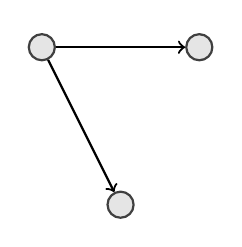
\begin{tikzpicture} 
            \tikzstyle{sentence}=[circle,thick,draw=black!75,fill=black!10,minimum size=2mm]
            \tikzstyle{edge}=[draw, thick,->]
            \begin{scope}
               \node [sentence] (s1) at (0,2) {\tiny{}};
               \node [sentence] (s2) at (2,2) {\tiny{}};
               \node [sentence] (s3) at (1,0) {\tiny{}}; 
               \path[edge] (s1) edge [above] node[font=\tiny] {} (s2);
               \path[edge] (s1) edge [above] node[font=\tiny] {} (s3);
            \end{scope}        
        \end{tikzpicture}
        & \rb{+0.43} & \rb{0.024}
        \\
        \midrule
        \rb{\emph{4-node}} &
        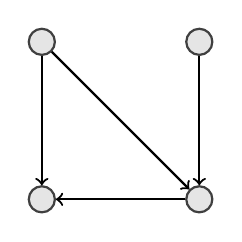
\begin{tikzpicture}
          \tikzstyle{sentence}=[circle,thick,draw=black!75,fill=black!10,minimum size=1mm]
          \tikzstyle{edge}=[draw, thick,->]
          \begin{scope}
              \node [sentence] (s1) at (0,2) {\tiny{}};
              \node [sentence] (s2) at (2,2) {\tiny{}};
              \node [sentence] (s3) at (2,0) {\tiny{}};
              \node [sentence] (s4) at (0,0) {\tiny{}};  
              \path[edge] (s1) edge [above] node[font=\tiny] {} (s3);
              \path[edge] (s1) edge [above] node[font=\tiny] {} (s4);
              \path[edge] (s2) edge [above] node[font=\tiny] {} (s3);
              \path[edge] (s3) edge [above] node[font=\tiny] {} (s4);
          \end{scope}        
        \end{tikzpicture}
        & \rb{-0.45} & \rb{0.018} \\
        &
        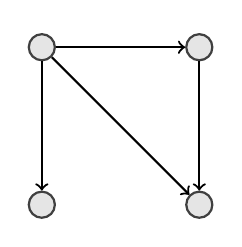
\begin{tikzpicture}
          \tikzstyle{sentence}=[circle,thick,draw=black!75,fill=black!10,minimum size=1mm]
          \tikzstyle{edge}=[draw, thick,->]
          \begin{scope}
             \node [sentence] (s1) at (0,2) {\tiny{}};
             \node [sentence] (s2) at (2,2) {\tiny{}};
             \node [sentence] (s3) at (2,0) {\tiny{}};
             \node [sentence] (s4) at (0,0) {\tiny{}};  
             \path[edge] (s1) edge [above] node[font=\tiny] {} (s2);
             \path[edge] (s1) edge [above] node[font=\tiny] {} (s3);
             \path[edge] (s1) edge [above] node[font=\tiny] {} (s4);
             \path[edge] (s2) edge [above] node[font=\tiny] {} (s3);
          \end{scope}        
        \end{tikzpicture}
      & \rb{+0.39} & \rb{0.047}\\
      &
      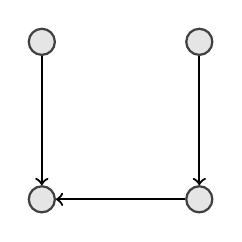
\begin{tikzpicture}
        \tikzstyle{sentence}=[circle,thick,draw=black!75,fill=black!10,minimum size=1mm]
        \tikzstyle{edge}=[draw, thick,->]
        \begin{scope}
           \node [sentence] (s1) at (0,2) {\tiny{}};
           \node [sentence] (s2) at (2,2) {\tiny{}};
           \node [sentence] (s3) at (2,0) {\tiny{}};
           \node [sentence] (s4) at (0,0) {\tiny{}};  
           \path[edge] (s1) edge [above] node[font=\tiny] {} (s4);
           \path[edge] (s2) edge [above] node[font=\tiny] {} (s3);
           \path[edge] (s3) edge [above] node[font=\tiny] {} (s4);
        \end{scope}        
      \end{tikzpicture}
      &  \rb{-0.43}  & \rb{0.024} \\ 
      &
      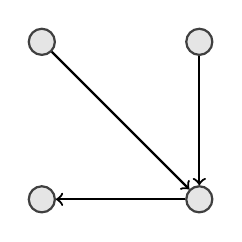
\begin{tikzpicture}
        \tikzstyle{sentence}=[circle,thick,draw=black!75,fill=black!10,minimum size=1mm]
        \tikzstyle{edge}=[draw, thick,->]
        \begin{scope}
           \node [sentence] (s1) at (0,2) {\tiny{}};
           \node [sentence] (s2) at (2,2) {\tiny{}};
           \node [sentence] (s3) at (2,0) {\tiny{}};
           \node [sentence] (s4) at (0,0) {\tiny{}};  
           \path[edge] (s1) edge [above] node[font=\tiny] {} (s3);
           \path[edge] (s2) edge [above] node[font=\tiny] {} (s3);
           \path[edge] (s3) edge [above] node[font=\tiny] {} (s4);
        \end{scope}        
      \end{tikzpicture}
      & \rb{-0.59} & \rb{0.001}\\
      &
      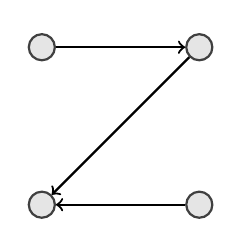
\begin{tikzpicture}
        \tikzstyle{sentence}=[circle,thick,draw=black!75,fill=black!10,minimum size=1mm]
        \tikzstyle{edge}=[draw, thick,->]
        \begin{scope}
           \node [sentence] (s1) at (0,2) {\tiny{}};
           \node [sentence] (s2) at (2,2) {\tiny{}};
           \node [sentence] (s3) at (2,0) {\tiny{}};
           \node [sentence] (s4) at (0,0) {\tiny{}};  
           \path[edge] (s1) edge [above] node[font=\tiny] {} (s2);
           \path[edge] (s2) edge [above] node[font=\tiny] {} (s4);
           \path[edge] (s3) edge [above] node[font=\tiny] {} (s4);
        \end{scope}        
      \end{tikzpicture}
      & \rb{-0.55} & \rb{0.003} \\
      &
      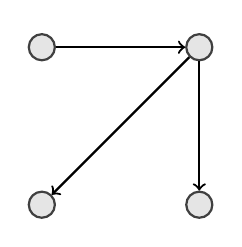
\begin{tikzpicture} 
        \tikzstyle{sentence}=[circle,thick,draw=black!75,fill=black!10,minimum size=1mm]
        \tikzstyle{edge}=[draw, thick,->]
        \begin{scope}
           \node [sentence] (s1) at (0,2) {\tiny{}};
           \node [sentence] (s2) at (2,2) {\tiny{}};
           \node [sentence] (s3) at (2,0) {\tiny{}};
           \node [sentence] (s4) at (0,0) {\tiny{}};  
           \path[edge] (s1) edge [above] node[font=\tiny] {} (s2);
           \path[edge] (s2) edge [above] node[font=\tiny] {} (s3);
           \path[edge] (s2) edge [above] node[font=\tiny] {} (s4);
        \end{scope}        
      \end{tikzpicture}
      & \rb{-0.55} & \rb{0.003}\\
      \bottomrule
    \end{tabular}
  \end{center}
  \caption{The Pearson correlation coefficient between frequencies of 3-node and \mbox{4-node}
  patterns that are significantly correlated with readability ratings that are assigned by human judges to texts in the \pitlerds dataset.}
  \label{tab:correlated-graphs}
\end{table}
%
Among all 3-node patterns, only the frequency of one pattern in the LexGraph representations of texts in this dataset is positively correlated with the readability ratings that are assigned by humans.  
Among the patterns with four nodes, frequencies of six patterns are significantly correlated with the readability ratings. 
The frequency of only one pattern is positively correlated, while the other five patterns are negatively correlated. 
Interestingly, both positively correlated 3-node and 4-node patterns have been determined as positively and significantly correlated with human readability ratings in experiments that are performed in the research presented in Chapter \ref{ch:coh-patterns}.
It indicates that our coherence model is linguistically sound.  

\section{Summary}
\label{sec:lex-graph-summary}

In the research presented in this chapter, we introduced a graph-based approach, named LexGraph, for representing the relations among sentences in a text based on the lexical relations among the words of sentences. 
We employ pre-trained word embeddings to identify lexical relations between words in sentences. 
This approach provides more informative graph representations of texts for coherence modeling in comparison to the entity graph representations of texts because the relations between sentences in LexGraph are not limited to coreference relation among entities. 
Relations in LexGraph are be built upon the semantic relations between any word pair in sentences. 
In this chapter, we extracted and counted subgraphs by a sampling approach for modeling coherence patterns and features. 


While the entity grid works only on sequences of up to two adjacent sentences, we can model relationships of up to six non-adjacent sentences. 
We solve the sparsity problem of large subgraphs by adapting \mbox{Kneser-Ney} smoothing to graphs. 
Smoothing prevents LexGraph from losing performance with large subgraphs.
It leads to superior performance on the \newcite{pitler08} dataset and to a first reasonable \mbox{state-of-the-art} on the \newcite{declercq14} dataset.

On the \pitlerds dataset, we achieve the best results to date.  
\newcite{pitler08} reported 83.25\% accuracy. 
In Chapter \ref{ch:coh-patterns}, by applying the idea of using frequency of subgraph as coherence features on the entity graph representation of texts, the model obtains 89.95\% accuracy. 
In the research of this chapter, by providing the lexical cohesion graph over sentences in texts and applying a smoothing method to frequencies of 5-node subgraphs, we could report 98.08\% accuracy. 
 These results, however, indicate that this dataset may not be the best one to report performance on and evaluate our coherence model. 
We observed that smoothing improves the performance of our coherence model on the \declercqds dataset as well. 


To conclude this chapter, the results of experiment presented in this chapter confirm our primary intuition that the capturing lexical relations among words in sentences via graphs is beneficial for coherence modeling. 
Applying the smoothing method on graphs of EGraph model increases the performance of this model. 
However, this improvement is not high as the improvement obtained on LexGraph.
These results show that our smoothing method is useful for both graph-based models, and our new graph representation, i.e.\ LexGraph, is more informative than the entity graph for coherence modeling. 

We summarize the contributions of this chapter as follows:

\begin{itemize}

  \item proposing a new \mbox{graph-based} representation of lexico-semantic relations across sentences,

  \item adapting the \mbox{Kneser-Ney} smoothing approach in order to solve the sparsity problem in frequency of large coherence patterns,  

  \item evaluating the model on two readability datasets: \newcite{pitler08} and \newcite{declercq14}.

\end{itemize}
